\chapter{Sovellus}
\label{ch:sovellus}

Rippikoulujen sisältö pohjautuu rippikoulusuunnitelmaan
\parencite{evlSuuriIhmeRippikoulusuunnitelma2017}, joka määrittää pääraamit
muun muassa sille kaikelle, mitä rippikoulussa käsitellään. Yksi rippikoulun
tärkeistä osaalueista on isoset ja heidän osallistumisensa ohjelman
suunnitteluun ja järjestämiseen. Rippikoulusuunnitelmassa
\parencite{evlSuuriIhmeRippikoulusuunnitelma2017} mainitaankin:

\begin{quotation}
    \noindent Isoset ovat tärkeä osa rippikoulun kokonaisuutta ja myös
    rippikoulun tiimiä. Siksi seurakunnan isostoimintaa ja rippikoulujen
    kokonaisuutta kannattaa suunnitella yhdessä. Isosilla on keskeinen rooli
    rippikoululaisten samastumiskohteina ja ”isosisaruksina”. Rippikoululaiset
    oppivat usein isosilta enemmän kuin ohjaajilta.
\end{quotation}

Rippikoulusuunnitelmassa tuodaan esille se, että eri paikkakunnilla ja eri
seurakunnilla on erilaiset mahdollisuudet järjestää asioita. Tässä työssä
tilannetta katsellaan erityisesti Ruokolahden seurakunnan isosten näkökulmasta.

Ruokolahden seurakunnalla rippikoulu koostuu muun muassa kirkkokäynneistä,
nuortenilloista, etätehtävistä, opetuspäivistä ja lopulta varsinaisesta
leiristä. Vuoden aikana isoskoulutusta käyvät isoset sekä aiempina vuosina
isoskoulutuksen käyneet osallistuvat järjestämään ohjelmaa vuoden aikana
käytäviin nuorteniltoihin sekä ovat avustamassa jumalanpalveluksissa sekä
opetuspäivissä. Nämä ovat yksittäisiä pienempiä asioita, jotka saadaan
yleensä järjestettyä pienemmällä määrällä. Varsinaisella leirillä kuitenkin
tahti on toisenlainen. Parin tunnin ohjelman sijaan leiriläisille luodaan koko
leirin ajaksi ohjelma, joka sisältää toimintaa heräämisestä hiljaisuuteen asti.
Tähän tiiviiseen ohjelmaan pakataan kaikki asiat, joita rippikoululla käydään
läpi. Ohjelmarunko ja opetus on suunniteltu etukäteen, mutta elää tilanteen
mukaan ja harvemmin pysyy alkuperäisessä edes yhtä kokonaista päivää. Ohjelman
ollessa tiivis ja muutosten tullessa tilanteen tarvittaessa erittäin lyhyellä
varoitusajalla ja rippikoulutiimin koostuessa yleensä noin neljästä aikuisesta,
kymmenestä isosesta sekä vierailijoista, kuten kanttorista ja diakonissasta,
on tärkeää, että kaikki ovat ajantasalla milloin mitäkin tapahtuu. Ruokolahden
seurakunnalla tähän käytettiin pitkään ensisijaisesti ja ainuana keinona yhtä
ryhmäkeskustelua, johon kuuluivat kaikki, jotka olivat läsnä leirillä. Leirin
ollessa viikon mittainen, oli viimeisinä päivinä viestien määrä tuhansissa ja
mediaa, kuten kuvia ja pdf:iä, useita satoja. Tällöin sisällön etsintä muuttui
yhä hankalammaksi viikkoa loppuun mennessä ja tiedotetut muutokset olivat
pitkälti muistin varassa.

Tämän työn ohessa on luotu sovellus, joka pyrkii tuomaan helpostusta edellä
kuvattuun tilanteeseen ja keventämään erityisten isosten työkuormaa, mutta
samalla myös ohjaajien. Tulevaisuudeen on mietitty myös mahdollisuutta luoda
mahdollisuus leiriläisille sekä huoltajille nähdä leiriin liittyviä asioita
sovelluksesta. Toistaiseksi sovellus on kuitenkin vain ohjaajien ja isosten
käytössä.

\section{Sovelluksen esittely}

Sovelluksesta löytyy kuvan \ref{fig:isosapp-leirit} mukaisesti kaikki leirit ja
leirien osallistujat, niin ohjaajat, isoset kuin leiriläisetkin. Leirillä
leiriläiset jaetaan leirillä isosryhmiin, jotka saadaan näkyviin leirin
päänykmään kuvassa \ref{fig:isosapp-ryhmat}.

\begin{figure}[h!]
    \centering
    \begin{minipage}[b]{.3\textwidth}
        \includegraphics[width=\textwidth]{figures/isosapp-leirit.png}
        \caption{Seurakunnan näkymä, joka sisältää leirit, ohjaajat ja isoset}
        \label{fig:isosapp-leirit}
    \end{minipage}\qquad
    \begin{minipage}[b]{.3\textwidth}
        \includegraphics[width=\textwidth]{figures/isosapp-ryhmat.png}
        \caption{Leirin päänäkymän ryhmä-osio}
        \label{fig:isosapp-ryhmat}
    \end{minipage}
\end{figure}

Sovellus pohjautuu ensisijaisesti aikatauluun, jonka ympärille kaikki muu
leiriin liittyvä toiminnallisuus on rakennettu. Leirin päänäkymässä kuvassa
\ref{fig:isosapp-nakkilista} on jokaiselle näkyvissä henkilökohtainen
tehtävälista, joka näyttää seuraavan 24 tunnin sisällä olevat ohjelmat, joissa
on vetovastuuna. Samassa näkymässä on myös niin sanottu nakkilista, joka
sisältää päivittäin vaihtuvat roolit isosille. Varsinainen aikataulu löytyy
omasta näkymästä, joka on nähtävissä kuvassa \ref{fig:isosapp-aikataulu}.

\begin{figure}[h!]
    \centering
    \begin{minipage}[b]{.3\textwidth}
        \includegraphics[width=\textwidth]{figures/isosapp-nakkilista.png}
        \caption{Leirin nakkilista ja henkilökohtainen tehtävälista}
        \label{fig:isosapp-nakkilista}
    \end{minipage}\qquad
    \begin{minipage}[b]{.3\textwidth}
        \includegraphics[width=\textwidth]{figures/isosapp-aikataulu.png}
        \caption{Leirin aikataulu ja ohjelmien vastuuhenkilöt}
        \label{fig:isosapp-aikataulu}
    \end{minipage}
\end{figure}

Näiden lisäksi ohjelman suunnittelua helpottamaan on luotu materiaalipankki,
josta löytyy kisoja, leikkejä ja sketsejä sekä listoja lauluista. Aikataulussa
oleviin ohjelmat on mahdollista linkittää suoraan materiaaliin, joten
ohjelmasta pääsee helposti näkemään mm. kilpailun säännöt, kuten kuvassa
\ref{fig:isosapp-materiaalit}. Materiaalin lisäksi ohjelman tekemisessä
tarvitaan välillä yksinkertaisia työkalua, kuten ryhmien arvontaa tai
telepromteria leikkimielisten uutisten lukemiseen. Näitä varten on luotu
kuvassa \ref{fig:isosapp-tyokalut} näkymä työkalu näkymä.

\begin{figure}[h!]
    \centering
    \begin{minipage}[b]{.3\textwidth}
        \includegraphics[width=\textwidth]{figures/isosapp-materiaalit.png}
        \caption{Esimerkki materiaaleihin lisätystä kilpailusta}
        \label{fig:isosapp-materiaalit}
    \end{minipage}\qquad
    \begin{minipage}[b]{.3\textwidth}
        \includegraphics[width=\textwidth]{figures/isosapp-tyokalut.png}
        \caption{Sovelluksen työkalu-näkymä}
        \label{fig:isosapp-tyokalut}
    \end{minipage}
\end{figure}

\clearpage
\section{Kielimallien integrointi osaksi sovellusta}

\begin{wrapfigure}{r}{0.45\textwidth}
    \centering
    \includegraphics[width=0.45\textwidth]{figures/isosapp-tyokalut-tarinan-generointi-1.png}
    \caption{Tarinan luontinäkymä}
    \label{fig:isosapp-tyokalut-tarinan-generointi-1}

    \qquad

    \includegraphics[width=0.45\textwidth]{figures/isosapp-tyokalut-tarinan-generointi-2.png}
    \caption{Sovelluksen työkalu-näkymä}
    \label{fig:isosapp-tyokalut-tarinan-generointi-2}
\end{wrapfigure}

Kielimallit ovat hyviä tuottamaan paljon sisältöä ja nopeasti. On tilanteita,
joissa tällaisesta on hyötyä, vaikka sisältöä ei olisikaan laadullisesti
parasta mahdollista. Yhtenä esimerkkinä tästä on työkalu, jolla saa generoitua
tarinaa. Tätä tarinaa voidaan käyttää pohjana muun muassa sketsien luomisessa.

Sovellukseen on toteutettu kielimalleja hyödyntävä työkalu, jolle saa valittua
käytettävän kielimallin ja annettua ohjeistuksen, mitä tarinan tulisi sisältää,
kuvan \ref{fig:isosapp-tyokalut-tarinan-generointi-1} mukaisesti.
Käyttöliittymä osaa näyttää tarinan vuorosanat sekä toiminnot, kuten kuvassa
\ref{fig:isosapp-tyokalut-tarinan-generointi-2} nähdään. Käyttöliittymä tukee
myös tarinan jatkamista mikäli vain valittulle kielimmallille on toteutettu
kyseinen toiminnallisuus backendin puolelle.

Työkalun lähtökohtana ollut päästä testaamaan useampaa eri kielimallia, joten
toteutuksesta on pyritty tekemään mahdollisimman joustava useammalla eri
kielimallille. Jokaisen kielimallin toteutuksen tulee toteuttaa
\ref{lst:StoryLineService.java} interfacen kaikki metodit, jotta kielimallia
saadaan käytettyä olemassa olevan käyttöliittymän kanssa. Metodit heittää
poikkeuksen, mikäli suoritus ei onnistunut, jolloin käyttöliittymä näyttää
virheen ja mahdollistaa uudelleen yrittämisen.

\clearpage
\begin{lstlisting}[
    basicstyle=\small,
    caption={StoryLineService interface, jonka toteuttamalla kielimallit saadaan },
    label={lst:StoryLineService.java},
    language=java,
]
public interface StoryLineService {

    List<StoryLine> createStoryLines(Story story);
    List<StoryLine> continueStoryLines(Story story);
    void cleanUp(Story story);
}
\end{lstlisting}

\subsection{Gemini toteutus}

Aiemmin kohdassa \ref{lst:GeminiServiceExample.java} esitelty GeminiService
saadaan käyttöön toteuttamalla StorylineService-interfacessa määritellyt
metodit tarinan luomiselle ja jatkamiselle esimerkin
\ref{lst:GeminiService.java} mukaisesti. Geminin kanssa on mahdollista käyttää
ChatSessionia, joka mahdollistaa viestien lähettämisen edestakaisin niin, että
kielimallilla on suoraan käytettävissä aiempi viestittely kontekstina. Tämän
ansiosta tarinaa on helppo jatkaa kunhan aiemmin luotu ChatSession on yhä
käytettävissä.

\begin{lstlisting}[
    basicstyle=\small,
    caption={Esimerkki GeminiServicen StorylineService-interfacen vaatimien metodien toteutuksesta},
    label={lst:GeminiService.java},
    language=java,
]
// Map, johon voidaan tallentaa luodut ChatSessionit myöhempää
// käyttöä varten
private final Map<UUID, ChatSession> chatSessions =
    new ConcurrentHashMap<>();

@Override
public List<StoryLine> createStoryLines(Story story) {
    // Luodaan ilmiintymä mallista ja avataan ChatSession
    GenerativeModel model = new GenerativeModel(
        story.getModelName().getName(),
        vertexAI
    );
    ChatSession chatSession = model.startChat();
    chatSession.withGenerationConfig(createGenerationConfig());

    // Tallennetaan ChatSession ConcurrentHashMap:iin, jotta tarinaa
    // saadaan jatkettua tarvittaessa helposti.
    chatSessions.put(story.getId(), chatSession);

    // Pyydetään luomaan tarina
    GenerateContentResponse response =
        chatSession.sendMessage(createInitializeContent(story));

    // Käsitellään vastaus
    return parseResponse(response);
}

@Override
public List<StoryLine> continueStoryLines(Story story) {
    // Tarkistetaan onko luotua tarinaa mahdollista jatkaa
    if (!chatSessions.containsKey(story.getId()))
        throw new GoneException();

    // Haetaan olemassa oleva ChatSession
    ChatSession chatSession = chatSessions.get(story.getId());

    // Pyydetään jatkamaan tarinaa
    GenerateContentResponse response =
        chatSession.sendMessage("Jatka tarinaa");

    // Käsitellään vastaus
    return parseResponse(response);
}

@Override
public void cleanUp(Story story) {
    // Poistetaan tallessa oleva ChatSession
    chatSessions.remove(story.getId());
}
\end{lstlisting}

Tarinan alustuksessa on annettu kielimallille sanallinen ohjeistus kohdan
\ref{lst:GeminiService.java::createInitializeContent} ja liitteen
\ref{ch:gemini-guide} mukaisesti, jossa on määritelty, missä muodossa vastaus
halutaan ja mitä vastauksen pitäisi sisältää. Ohjeistukseen on liitetty
käyttäjän antama syöte käyttöliittymästä.

\begin{lstlisting}[
    basicstyle=\small,
    caption={Geminin ohjeistuksen luominen},
    label={lst:GeminiService.java::createInitializeContent},
    language=java,
]
private Content createInitializeContent(Story story) {
    String guide = "..."; // Liittestä löytyvä ohjeistus

    // Yhdistetään käyttäjän antama kuvaus ja ohjeistus tulosteesta
    return ContentMaker.fromString(story.getText() + "\n\n" + guide);
}
\end{lstlisting}

Gemini osaa tuottaa sanallisen ohjeistuksen mukaisesti vastauksen suoraan JSON-
muodossa, jolloin se pystytään parsimaan ilman, että vastausta tarvitsee
käsitellä sen enempää. Vastauksen parsiminen saadaan siis toteutettu hyvinkin
yksinkertaisesti esimerkin \ref{lst:GeminiService.java::parseResponse}
mukaisesti.

\begin{lstlisting}[
    basicstyle=\small,
    caption={Geminin vastausten käsittely},
    label={lst:GeminiService.java::parseResponse},
    language=java,
]
private List<StoryLine> parseResponse(GenerateContentResponse response)
    throws JsonProcessingException
{
    // Luetaan vastauksen teksti
    String text = response.getCandidates(0)
        .getContent()
        .getParts(0)
        .getText();

    // Parsitaan luettu json-teksti listaksi StoryLine-ilmiintymiä
    return objectMapper.readValue(text, new TypeReference<>() {});
}
\end{lstlisting}

Toteutuksen jälkeen kielimallia voidaan käyttää tuottamaan kuvassa
\ref{fig:isosapp-tyokalut-tarinan-generointi-2} näkyvä tarina kuvan
\ref{fig:isosapp-tyokalut-tarinan-generointi-1} käyttöliittymän
toiminnallisuudella.

\subsection{PaLM2 toteutus}

Vastaavasti \ref{lst:PaLM2Service.java} kohdassa esitelty PaLM2Service saadaan
toteuttamaan StorylineService-interface esimerkin
\ref{lst:PaLM2Service.java::createStoryLines} mukaisesti. PaLM 2:lle ei ole
tarjolla vastaavaa ChatSessionia, kuin Geminille, joten on sille toteutettu
vain tarinan luonti, muttei mahdollisuutta jatkaa tarinaa.

\begin{lstlisting}[
    basicstyle=\small,
    caption={Esimerkki PaLM2Servicen StorylineService-interfacen metodien toteutuksesta},
    label={lst:PaLM2Service.java::createStoryLines},
    language=java,
]
@Override
public List<StoryLine> createStoryLines(Story story) {
    // Tehdään pyyntö kielimallille
    PredictResponse predictResponse = vertexAI
        .getPredictionServiceClient()
        .predict(PredictRequest.newBuilder()
            .setEndpoint(
                getEndpointName(story.getModelName().getName())
                .toString())
            .addInstances(getPrompt(generatePrompt(story)))
            .setParameters(getParameters())
            .build());

    // Käsitellään vastaus
    return parseResponse(response);
}
\end{lstlisting}

PaLM2-kielimallille on luotu vastaava ohjeistuis kuin Geminille, jossa
määritellään minkälainen vastaus kielimallin tulisi tuottaa ja kielimallille
annetaan käyttäjän antama syöte. Ohjeistuksen toteutus on nähtävissä kohdassa
\ref{lst:PaLM2Service.java::generatePrompt} ja koko ohjeistus liitteessä \ref{ch:palm2-guide}.

\begin{lstlisting}[
    basicstyle=\small,
    caption={PaLM2 ohjeistuksen luonti},
    label={lst:PaLM2Service.java::generatePrompt},
    language=java,
]
private String generatePrompt(Story story) {
    String guide = "..."; // Liitteestä löytyvä ohjeistus

    // Yhdistetään käyttäjän antama syöte ja ohjeistus
    return story.getText() + "\n\n" + guide;
}

// Apufunktio ohjeistuksen muuttamiseen kielimallin haluamaan muotoon
private com.google.protobuf.Value getPrompt(String prompt) throws
    InvalidProtocolBufferException, JsonProcessingException
{
    Map<String, Object> instance = new HashMap<>();
    instance.put("prompt", prompt);
    return convertMapToValue(instance);
}
\end{lstlisting}

PaLM2:sta ohjeistaessa sanallisesti, että tuloksen tulee olla JSON-muodossa,
tulee tuloste Markdownin tukemassa JSON-muodossa, jossa varsinanen JSON osuus
on ympäritöity JSON-koodiosiota tarkoittavilla merkinnöillä. Jotta tulos
saadaan käsitelty, tulee vastauksesta saada nämä pois. Tämä saadaan toteutettua
esimerkin \ref{lst:PaLM2Service.java::parseResponse} mukaisesti.

\begin{lstlisting}[
    basicstyle=\small,
    caption={PaLM2 vastauksen käsittely},
    label={lst:PaLM2Service.java::parseResponse},
    language=java,
]
private List<StoryLine> parseResponse(PredictResponse response)
    throws JsonProcessingException
{
    String json = response
        .getPredictions(0)
        .getStructValue()
        .getFieldsOrThrow("content")
        .getStringValue()
        .replaceFirst("```json\n", "")
        .replaceFirst("```", "");

    return objectMapper.readValue(json, new TypeReference<>() {});
}
\end{lstlisting}

\subsection{Llama 3 toteutus}

Kun Llama 3:sta käytetään VertexAI:n tarjoaman kirjaston kautta, tukee se
samoja toimintoja, kuin mitä on käytetty Geminin toteutuksessa. Toteutus
saadaan tällöin tehtyä samanlaisena kuin Geminillä kohdassa
\ref{lst:GeminiService.java}.

Kielimallille annettava ohjeistus eroaa kuitenkin siitä, mitä Geminille
annetaan. Ohjeistus saadaan luotua vastaavasti kuin Geminille kohdassa
\ref{lst:GeminiService.java::createInitializeContent}, mutta ohjeistuksena
annettava teksti on liitteessä \ref{ch:llama3-guide}. Ohjeistus on vastaava
kuin PaLM2:lla, mutta kielimallille tuli erikseen sanoa, että tulosteessa ei
saa olla muuta kuin JSON-vastaus, jotta kielimalli jätti ylimääräisen
tulosteen pois ja tuotti vain halutun tuloksen.

\subsection{xAI:n toteutus}

XAI:n rajapinnan dokumentaatiossa on määritelty 'response\_format'-kenttä, mutta
kyseiselle kentälle ei ole määritelty tyyppiä \parencite{xAIDocsEndpoints}.
Mahdollinen formaatti kyseiselle kentälle löydetään Githubissa olevasta
issuesta \parencite{githubBerriAIlitellmIssues6610}, jossa ongelmana on se,
ettei vastauksen formatointi ole tuettu sillä hetkellä. Testaamalla samalla
formaatilla saamme itsekkin vastauksena kohdassa \ref{lst:xai-bad-request.json}
näkyvän virheviestin ettei ainakaan kyseinen formatointi ole käytössä.

\begin{lstlisting}[
    basicstyle=\small,
    caption={XAI rajapinnan palauttama vastaus, kun yritetään määrittää 'response\_format'-kenttä},
    label={lst:xai-bad-request.json},
]
{
    "code":"Client specified an invalid argument",
    "error":"The model does not support formatted output but some
      have been specified in the request."
}
\end{lstlisting}

Vaikkei rajapinta suoraan vaikuta tukevan vastauksen muotoilua, voidaan ohjeet
muotoiluun antaa kirjallisesti. Alustamalla keskustelu system-roolilta
tulevalla viestillä:

\begin{quotation}
    \noindent Olet käsikirjoittaja. Luot tarinan käyttäjän antaman syötteen
    perusteella.

    \noindent Vastauksesi tulee olla JSON-muodossa oleva lista, joka koostuu
    olioista, joilla on kolme attribuuttia: type, target ja content. Type voi
    olla joko `ACTION` tai `TALK` riippuen siitä, onko kyseessä jotakin mitä
    tapahtuu vai jotain mitä joku sanoo. Target kuvastaa sitä kuka tekee tai
    kuka sanoo. Content kuvastaa sitä mitä tapahtuu tai sanotaan.
\end{quotation}

saadaan vastaukset halutussa JSON-muodossa, jonka myötä saadaan viesti
parsittua StoryLineService-interfacen metodien vastauksien haluamaan
muotoon antamalla vastaus suoraan JSON-parserille kohdan
\ref{lst:XAIService.java::parseResponse} mukaisesti.

\begin{lstlisting}[
    basicstyle=\small,
    caption={XAI rajapinnan palauttaman vastauksen parsiminen haluttuun muotoon},
    label={lst:XAIService.java::parseResponse},
    language=java,
]
private List<StoryLine> parseResponse(Message message)
    throws IOException
{
    // Luetaan viestin sisältö ja poistetaan ylimääräinen muotoilu
    String json = message.content()
        .replaceFirst("```json\n", "")
        .replaceFirst("```", "");

    // Luetaan tekstimuodossa oleva json listaksi StoryLine-olioita
    return objectMapper.readValue(json, new TypeReference<>() {});
}
\end{lstlisting}

Käytettävä rajapinta päätepiste pohjautuu alunperinkin siihen, että sinne
lähetetään lista viesteistä. Tätä hyödyntämällä pystymme toteuttamaan
toiminnallisuuden tarinan jatkamiseen. Pitämällä kirjaa aiemmista viesteistä
voimme tarinan jatkamisessa yksinkertaisesti hakea vanhat viestit ja pyytää
jatkamaan tarinaa kuten kohdassa \ref{lst:XAIService.java::continueStoryLines}
olevassa toteutuksessa on tehty.

\begin{lstlisting}[
    basicstyle=\small,
    caption={XAI rajapinnan palauttaman vastauksen parsiminen haluttuun muotoon},
    label={lst:XAIService.java::continueStoryLines},
    language=java,
]
public List<StoryLine> continueStoryLines(Story story) {
    // Haetaan keskustelun vanhat viestit
    List<Message> messages = chats.get(story.getId());

    // Tarkistetaan ettei tarina kasva liian pitkäksi
    if (story.getLines().size() > 50 || messages.size() > 10)
        throw new BadRequestException("Tarina on liian pitkä!");

    // Lisätään käyttäjän pyyntö jatkaa tarinaa
    messages.add(new Message("user", "Jatka tarinaa"));

    // tehdään pyyntö
    // parsitaan vastaus
    // palautetaan uudet rivit
}
\end{lstlisting}

\section{Kielimallien toimivuuden arviointia}

Lopputuloksen ollessa tarina, jota mahdollisesti voidaan hyödyntää
ohjelmanumeroiden kehittämisessä, on sen varsinaisen tulosteen laadun arviointi
hankalaa. Työ on kuitenkin keskittynyt enemmän siihen, miten yksinkertaisesti,
helposti, nopeasti ja edullisesti saadaan toteutettua haluttu toiminnallisuus
ilman ylimääräistä työtä ja hienosäätöä. Tällöin arvioinnin kannalta oleellista
onkin se, että toimiko ratkaisu ylipäätänsä jotenkin.

Vuoden 2025 alkupuolella sovellukseen integroiduista kielimalleista ainoastaan
Gemini ja Llama3 olivat enää toiminnassa, joten toimivuuden arvioinnissa
käytettiin vain näitä kielimalleja. Suurin syy muiden kielimallien
toimimattomuuden oli rajapintojen kielteiset vastaukset puuttuvien krediittien
takia.

Arvointi toteutettiin yksinkertaisella testillä, jossa luotiin kuusi syötettä,
jotka annettiin jokaiselle kielimallille 5 kertaa ja yritettiin jokaisella
kerralla jatkaa tarinaa 5 kertaa. Annettuja syötteitä olivat seuraavat:

\begin{quotation}
    \noindent Kerro tarina opiskelijoista kouluruokailussa

    \noindent Kerro tarina kavereista matkalla elokuviin

    \noindent Kerro tarina opiskelijabileistä

    \noindent Kerro tarina työkavereista viettämässä pikkujouluja

    \noindent Kerro tarina jalkapallojoukkueesta matkalla kisoihin

    \noindent Kerro tarina leiriläisistä riparilla
\end{quotation}

Onnistuneet tarinan generoinnin määrät ovat nähtävissä graaffissa
\ref{chart:story-start}. Onnistumiseksi laskettiin se, että tarinaan saatiin
tuotettuja rivejä, kun puolestaan epäonnistumiseksi se, että käyttöliittymä
näytti virheilmoituksen. Teoriassa käyttöliittymä voisi näyttää virhetilanteita
muitakin kuin kielimallien integraatiosta liittyvistä syistä, kuten verkko-
ongelmista, mutta testin aikana tällaisia virheitä ei havaittu.

\begin{figure}[H]
    \centering
    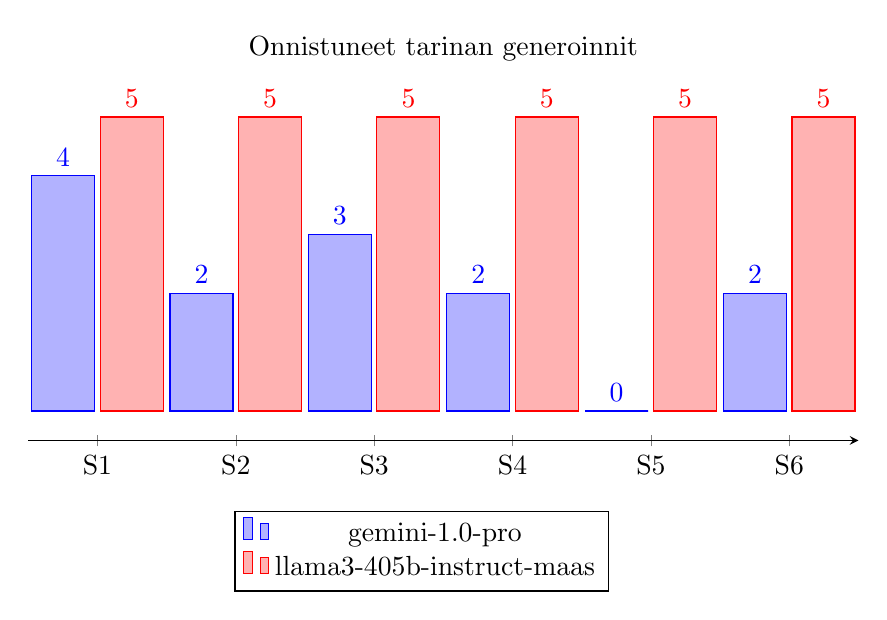
\begin{tikzpicture}
        \begin{axis}[
            ybar,
            bar width=0.8cm,
            width=\textwidth,
            height=.5\textwidth,
            title={Onnistuneet tarinan generoinnit},
            symbolic x coords={S1, S2, S3, S4, S5, S6},
            legend style={at={(0.7,-0.2)}},
            axis y line=none,
            axis x line=bottom,
            nodes near coords,
            enlargelimits=0.1,
            xtick=data,
            enlarge x limits=auto,
        ]
        \addplot+ coordinates {(S1, 4) (S2, 2) (S3, 3) (S4, 2) (S5, 0) (S6, 2)};
        \addplot+ coordinates {(S1, 5) (S2, 5) (S3, 5) (S4, 5) (S5, 5) (S6, 5)};
        \legend{gemini-1.0-pro,llama3-405b-instruct-maas}
        \end{axis}
    \end{tikzpicture}
    \caption{Onnistuneiden tarinan generointien määrät annettua syötettä kohden}
    \label{chart:story-start}
\end{figure}

Taulukon \ref{chart:story-start} tuloksista huomataan, että Llama3 onnistui
joka kerta generoimaan tarinan kun Geminin onnistuminen vaihteli huomattavasti.
Järjestelmän logien karkean läpikäynti paljasta pääasialliseksi ongelmaksi
Geminin kanssa sen, että syötteessä oli jotain muuta kuin haluttu JSON-
muotoinen vastaus. Osan kerroista pyyntö oli markdowia, osan puolestaan katkesi
kesken kaiken. Molemmat ovat tilanteita, jotka olisi mahdollista korjata melko
yksinkertaisesti tuloksen kesittelyyn, jolloin Gemini voisi päästä lähelle tai
jopa täysin samoihin tuloksiin kuin Llama3.

Sekä Gemini, että Llama3 tukivat molemmat tarinan jatkamista, joten tarinoita
yritettiin jatkaa tarinan luonnin jälkeen 5 kertaa. Näistä laskettiin
onnistuneet kerrat. Mikäli tarinan luonti epäonnistui jo alunperin, tarkoitti
se tarinan jatkamisen kannalta suoraan sitä, että tarinan jatkaminen onnistui
0 kertaa. Käyttöliittymä mahdollista virheen jälkeen sen, että tarinaa
yritettäisiin yhä jatkaa. Tätä ei kuitenkaan tehty sillä kielimallin kanssa
käyty keskustelu sisälsi tällöin virhetilanteessakin luodun osan, joka ei
näkynyt käyttäjälle, mutta oli kielimallille tiedossa, joten tarinan
yhtenäisyys kärsi jokaisesta virheestä. Määrät onnistuneista tarinan
jatkamisista ovat nähtävissä graaffissa \ref{chart:story-continue}. Tarinan
jatkamisessa Geminin kohdanneet ongelmat olivat vastaavia kuin tarinan
luonnissa.

\begin{figure}[H]
    \centering
    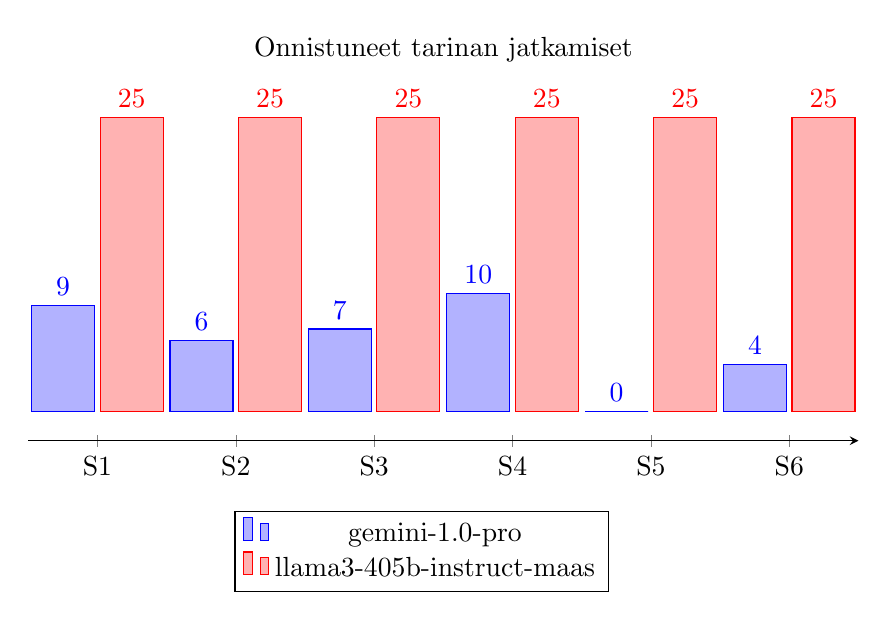
\begin{tikzpicture}
        \begin{axis}[
            ybar,
            bar width=0.8cm,
            width=\textwidth,
            height=.5\textwidth,
            title={Onnistuneet tarinan jatkamiset},
            symbolic x coords={S1, S2, S3, S4, S5, S6},
            legend style={at={(0.7,-0.2)}},
            axis y line=none,
            axis x line=bottom,
            nodes near coords,
            xtick=data,
            enlarge x limits=auto,
        ]
        \addplot+ coordinates {(S1, 9) (S2, 6) (S3, 7) (S4, 10) (S5, 0) (S6, 4)};
        \addplot+ coordinates {(S1, 25) (S2, 25) (S3, 25) (S4, 25) (S5, 25) (S6, 25)};
        \legend{gemini-1.0-pro,llama3-405b-instruct-maas}
        \end{axis}
    \end{tikzpicture}
    \caption{Onnistuneiden tarinan jatkamisien määrät aiemmin annettujen syötteiden pohjalta luoduille tarinoille}
    \label{chart:story-continue}
\end{figure}

Jokaiselle onnistuneelle tarinan generoinnille laskettiin rivimäärä, joka
sisältää sekä vuorosanat että toiminnan. Graaffista \ref{chart:story-lines} on
nähtävissä keskimääräiset määrät tuotetuille riveille.

\begin{figure}[H]
    \centering
    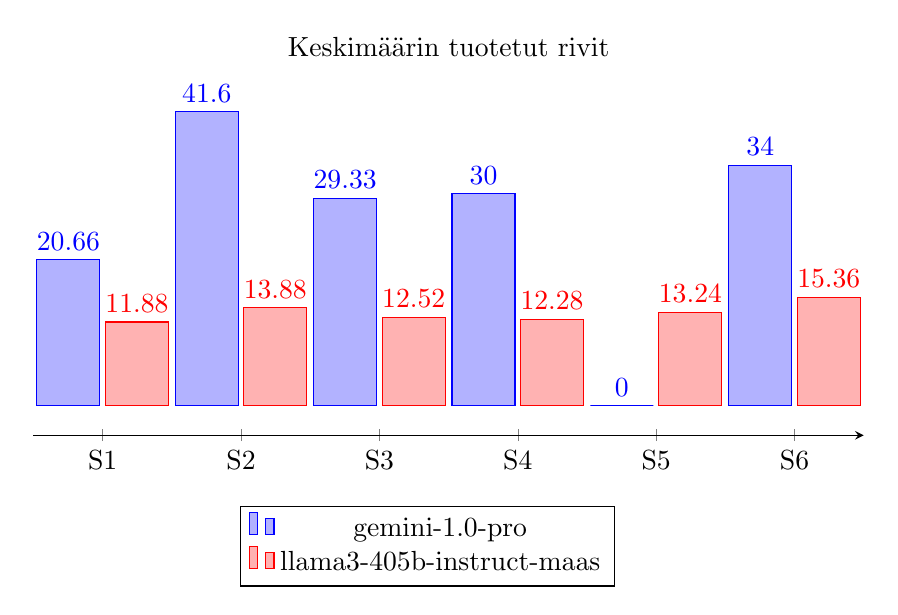
\begin{tikzpicture}
        \begin{axis}[
            ybar,
            bar width=0.8cm,
            width=\textwidth,
            height=.5\textwidth,
            title={Keskimäärin tuotetut rivit},
            symbolic x coords={S1, S2, S3, S4, S5, S6},
            legend style={at={(0.7,-0.2)}},
            axis y line=none,
            axis x line=bottom,
            nodes near coords,
            xtick=data,
            enlarge x limits=auto,
        ]
        \addplot+ coordinates {(S1, 20.66) (S2, 41.6) (S3, 29.33) (S4, 30) (S5, 0) (S6, 34)};
        \addplot+ coordinates {(S1, 11.88) (S2, 13.88) (S3, 12.52) (S4, 12.28) (S5, 13.24) (S6, 15.36)};
        \legend{gemini-1.0-pro,llama3-405b-instruct-maas}
        \end{axis}
    \end{tikzpicture}
    \caption{Keskimäärin tuotettujen rivien määrä onnistuneissa pyynnöissä}
    \label{chart:story-lines}
\end{figure}

Testien tuloksien pohjalta Llama3 vaikutti suorituvan tasaisen varmasti tarinan
generoinnista, mutta Gemini puolestaan sai tuotettua enemmän tarinaa yhdellä
kertaa. Testaamisen yhteydessä lisäksi Llama3 toimi erittäin hitaasti
verrattuna Gemininiin. Tätä ei kuitenkaan mitattu vaan pohjautuu puhtaasti
testin tekijän käsitykseen tilanteesta. Geminin toimintaa testattiin myös lähes
vuosi aiemmin isosten toimesta sovellusken julkaisuhetkellä. Tuolloin isoset
eivät tuoneet esille läheskään yhtä isoa määrää virhetilanteita kuin mitä
varsinaisessa testissä tuli. Tällöin kuitenkin lähinnä keskityttiin yleiseen
mielipiteeseen ja isoimpiin puutteisiin sekä ohjelmistovirheisiin joita tuli
esille sovelluksessa itsessään, eikä tuolta ajalta ole statistiikkaa, jota
voisi verrata tuoreempiin mittauksiin.

Mittaustulosten käsittelyhetkellä Geministä oli saatavilla huomattavasti
uudempi ja kyvykkäämpi malli, joka olisi voinut olla mahdollisesti
tasapuolisempi vertailuun Llama3:n isoimman mallin kanssa. \parencite{gemini2}
